\chapter{Class Diagrams}

\section{First Cycle Design}
\label{sec:appendix1}
  \begin{figure}[!htb]
    \begin{center}
      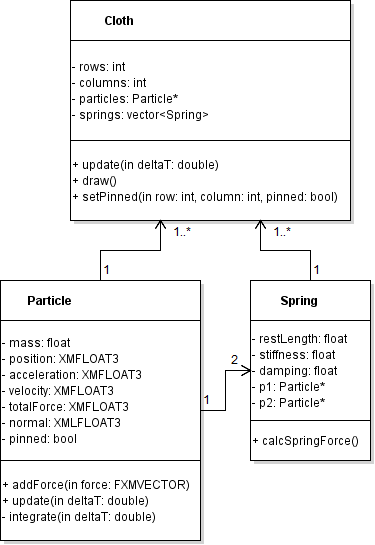
\includegraphics[scale=0.66]{Figures/cycle_1_initial_design}
    \end{center}
    \caption{Initial design for the first development cycle}
    \label{fig:phase1 initial}
  \end{figure}
  
  \begin{figure}
    \begin{center}
      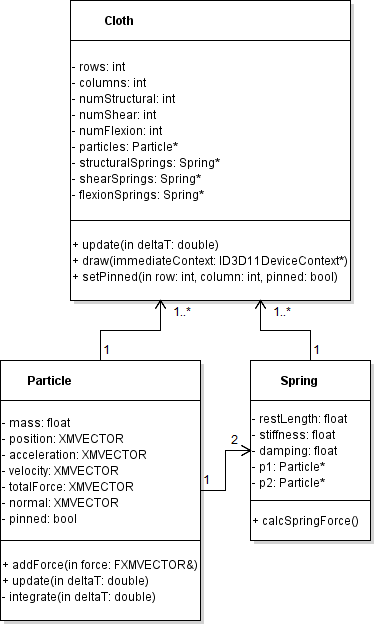
\includegraphics[scale=0.66]{Figures/cycle_1_final_design}
    \end{center}
    \caption{Final design for the first development cycle}
    \label{fig:phase1}
  \end{figure}
  
\begin{landscape}
\section{Second Cycle Design}
  \begin{figure}[!htb]
    \begin{center}
      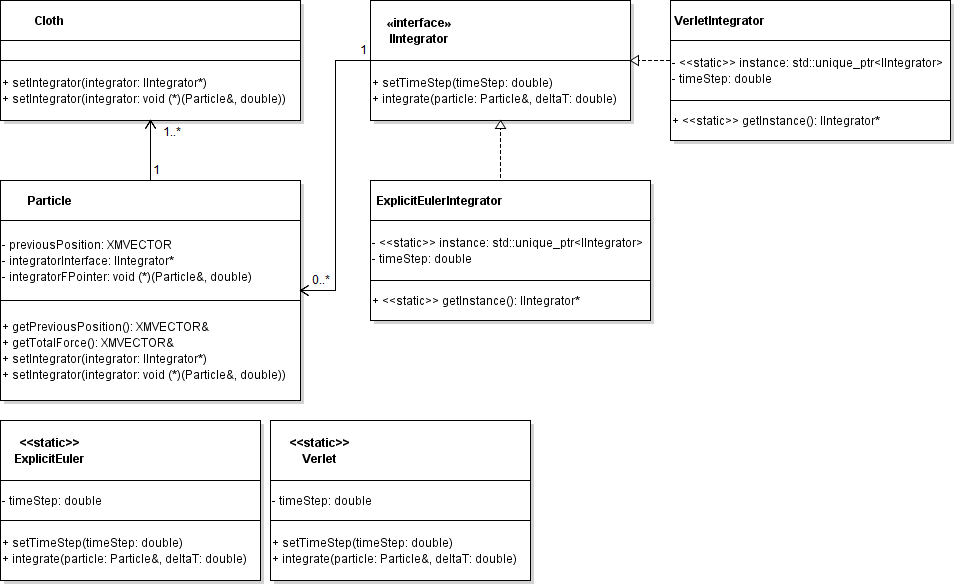
\includegraphics[scale=0.63]{Figures/cycle_2_initial_design}
    \end{center}
    \caption{Initial design for the second development cycle}
    \label{fig:phase2 initial}
  \end{figure}
  
  \begin{figure}
    \begin{center}
      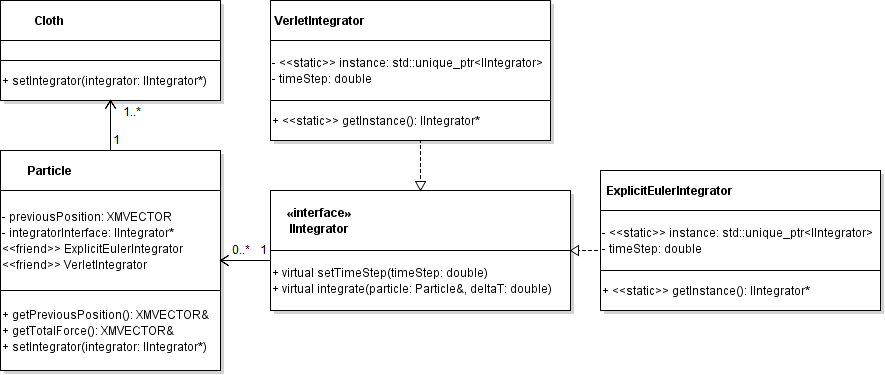
\includegraphics[scale=0.75]{Figures/cycle_2_final_design}
    \end{center}
    \caption{Final design for the second development cycle}
    \label{fig:phase2}
  \end{figure}
\end{landscape}

\section{Third Cycle Design}
  \begin{figure}[!htb]
    \begin{center}
      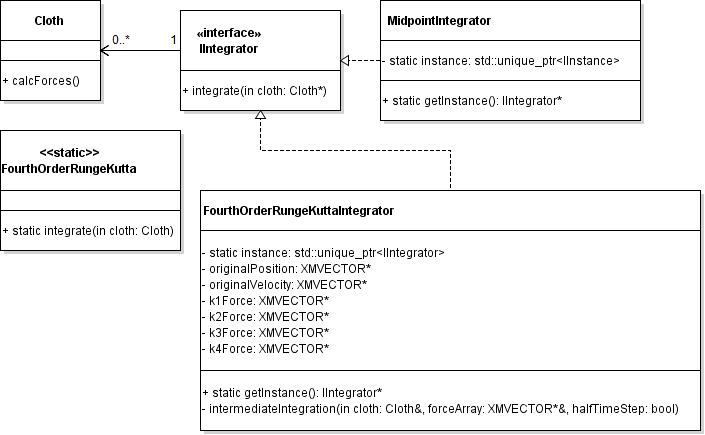
\includegraphics[scale=0.70]{Figures/cycle_3_initial_design}
    \end{center}
    \caption{Initial design for the third development cycle}
    \label{fig:phase3 initial}
  \end{figure}
  
  \begin{figure}
    \begin{center}
      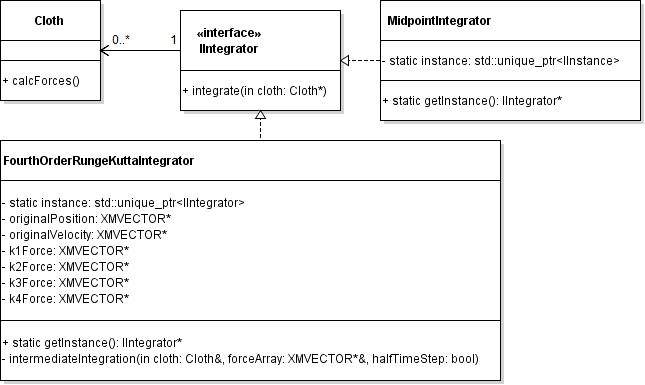
\includegraphics[scale=0.75]{Figures/cycle_3_final_design}
    \end{center}
    \caption{Final design for the third development cycle}
    \label{fig:phase3}
  \end{figure}

\begin{landscape}
\chapter{Profiling Results}

\section{First Cycle}
  \begin{figure}[!htb]
    \begin{center}
      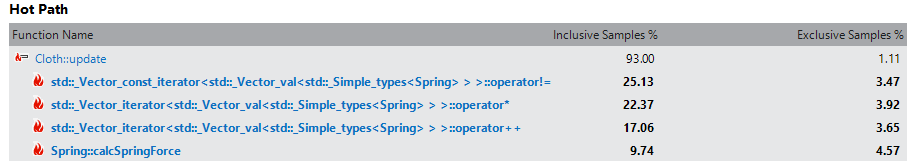
\includegraphics[scale=1.0]{Figures/vector_profiling_before}
    \end{center}
    \caption{Profiling results using a std::vector to store springs}
    \label{fig:profiling1}
  \end{figure}
  
    \begin{figure}
    \begin{center}
      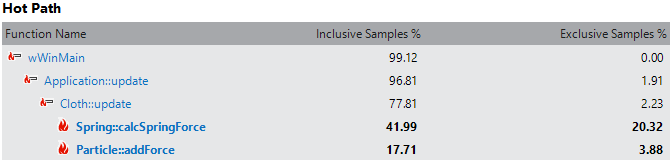
\includegraphics[scale=1.0]{Figures/vector_profiling_after}
    \end{center}
    \caption{Profiling results using dynamic arrays to store springs}
    \label{fig:profiling2}
  \end{figure}
  
    \begin{figure}[!htb]
    \begin{center}
      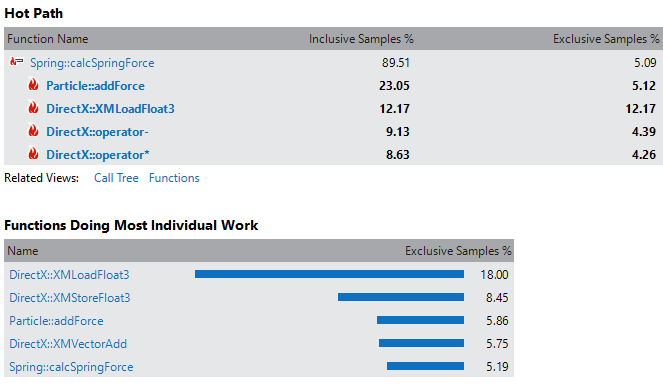
\includegraphics[scale=1.0]{Figures/calcspringforce_profiling_before}
    \end{center}
    \caption{Profiling results for unoptimised calcSpringForce}
    \label{fig:profiling3}
  \end{figure}
  
    \begin{figure}[!htb]
    \begin{center}
      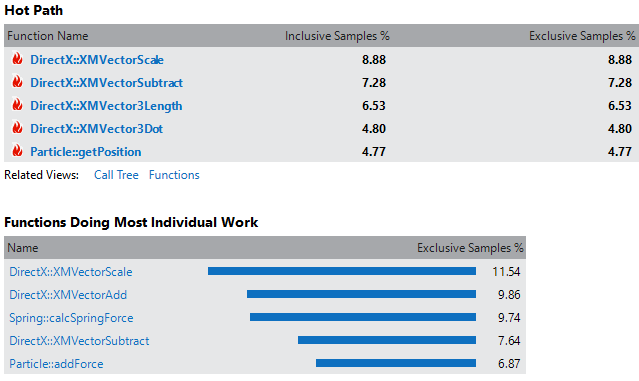
\includegraphics[scale=1.0]{Figures/calcspringforce_profiling_after}
    \end{center}
    \caption{Profiling results for optimised calcSpringForce}
    \label{fig:profiling4}
  \end{figure}
\end{landscape}

\begin{landscape}
\chapter{Test Results}

\section{Explicit Euler}

\subsection{Sheet Data}

  \begin{figure}[!htb]
    \begin{center}
      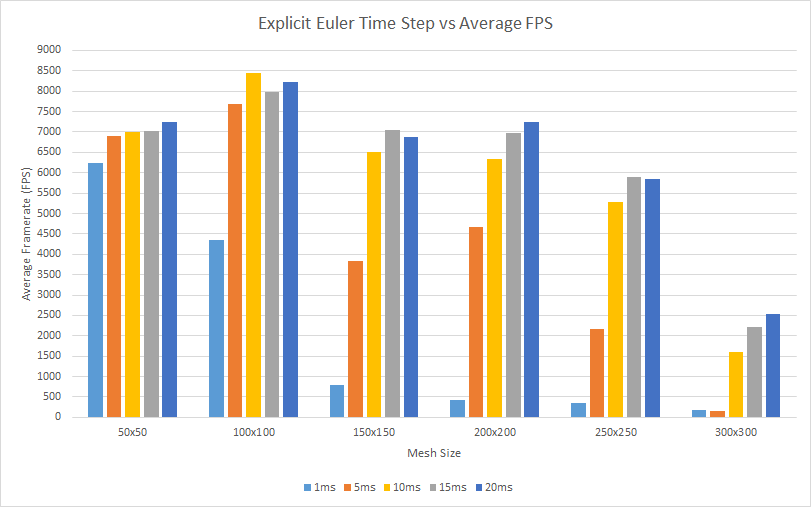
\includegraphics{Figures/sheet_ee_fps}
    \end{center}
    \caption{Explicit Euler time step against average FPS (sheet)}
    \label{fig:ee fps sheet}
  \end{figure}
\end{landscape}
  
    \begin{figure}
    \begin{center}
      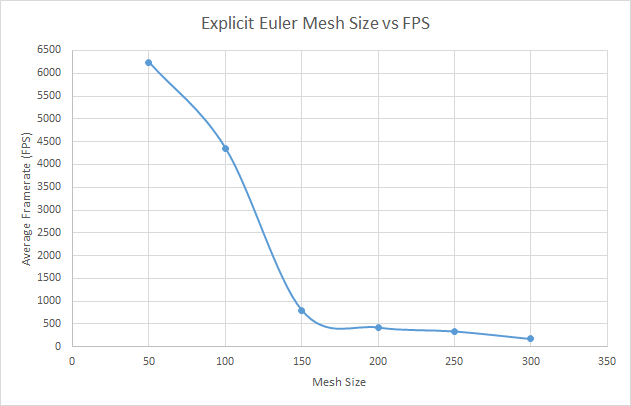
\includegraphics[scale=.9]{Figures/sheet_ee_m_fps}
    \end{center}
    \caption{Explicit Euler mesh size against average FPS (sheet)}
    \label{fig:ee mesh fps sheet}
  \end{figure}
  
    \begin{figure}
    \begin{center}
      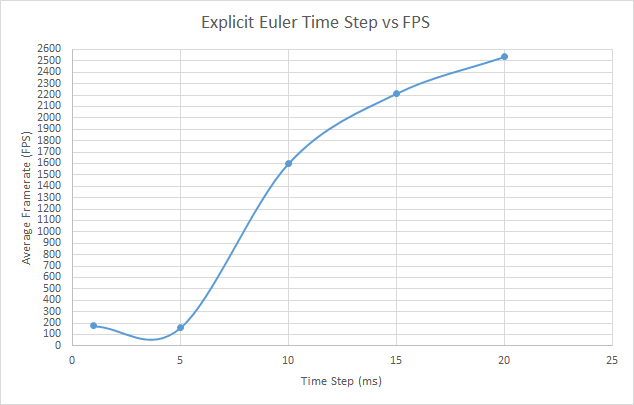
\includegraphics[scale=.9]{Figures/sheet_ee_ts_fps}
    \end{center}
    \caption{Explicit Euler time step against average FPS for a 300 by 300 mesh (sheet)}
    \label{fig:ee step fps sheet}
  \end{figure}
  
    \begin{figure}
    \begin{center}
      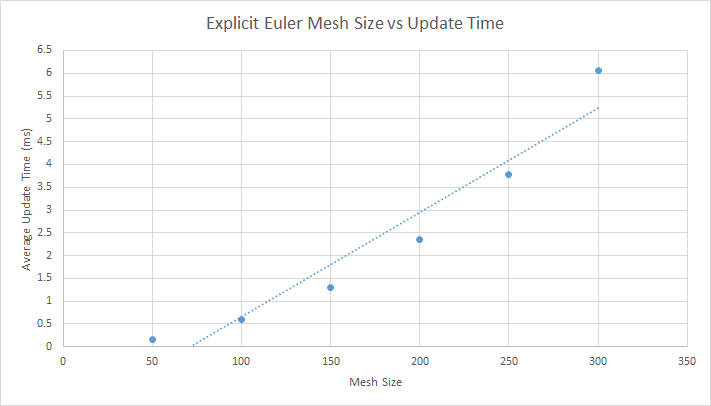
\includegraphics[scale=.9]{Figures/sheet_ee_m_ut}
    \end{center}
    \caption{Explicit Euler mesh size against average update time (sheet)}
    \label{fig:ee mesh update sheet}
  \end{figure}
  
    \begin{figure}
    \begin{center}
      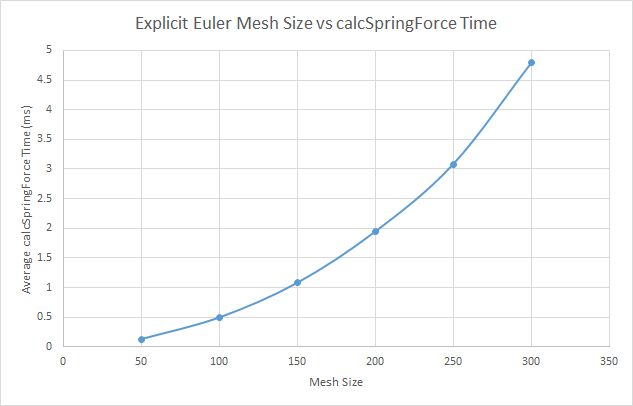
\includegraphics[scale=.9]{Figures/sheet_ee_m_csf}
    \end{center}
    \caption{Explicit Euler mesh size against average internal force time (sheet)}
    \label{fig:ee mesh csf sheet}
  \end{figure}
  
    \begin{figure}
    \begin{center}
      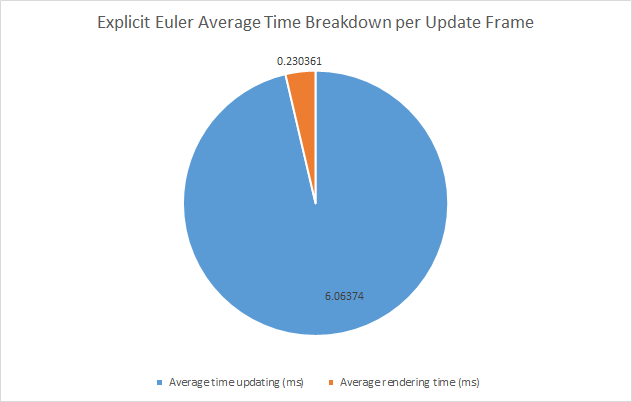
\includegraphics[scale=.9]{Figures/sheet_ee_ft}
    \end{center}
    \caption{Explicit Euler frame time breakdown (sheet)}
    \label{fig:ee ft sheet}
  \end{figure}
  
    \begin{figure}
    \begin{center}
      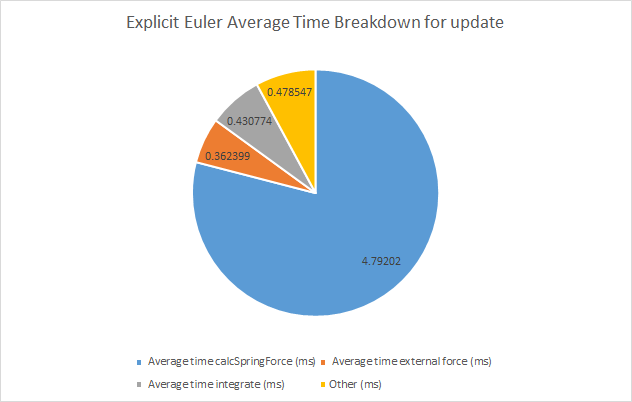
\includegraphics[scale=.9]{Figures/sheet_ee_ut}
    \end{center}
    \caption{Explicit Euler update time breakdown (sheet)}
    \label{fig:ee ut sheet}
  \end{figure}

\begin{landscape}
\subsection{Flag Data}

    \begin{figure}[!htb]
    \begin{center}
      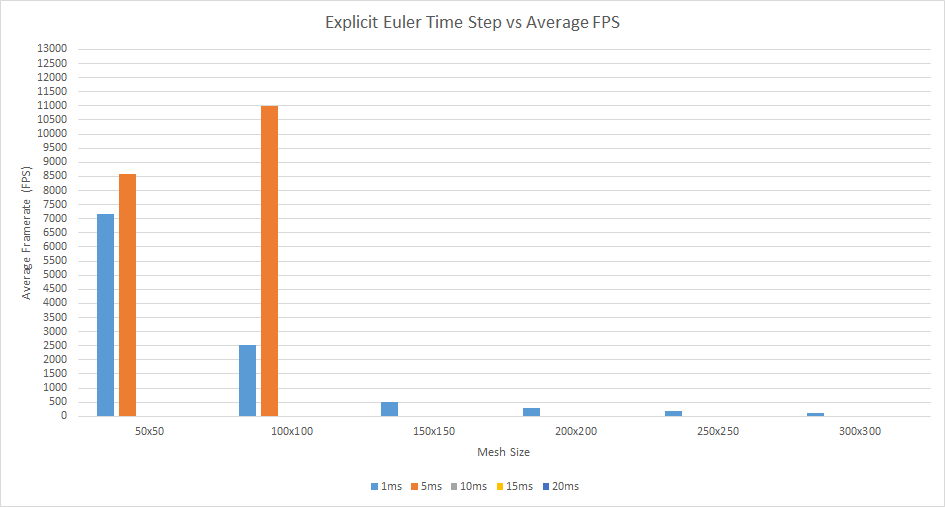
\includegraphics[scale=0.95]{Figures/flag_ee_fps}
    \end{center}
    \caption{Explicit Euler mesh size against average FPS (flag)}
    \label{fig:ee fps flag}
  \end{figure}
\end{landscape}
  
    \begin{figure}
    \begin{center}
      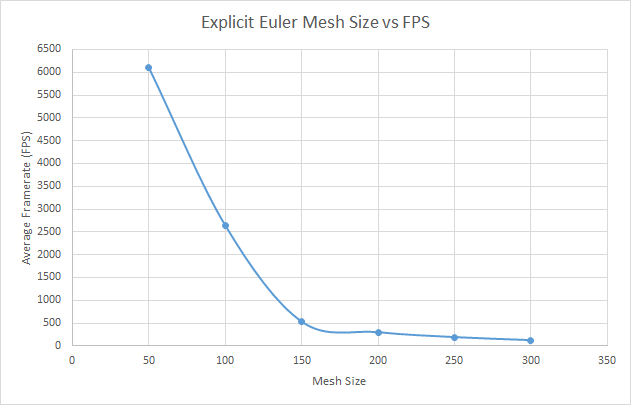
\includegraphics[scale=.9]{Figures/flag_ee_m_fps}
    \end{center}
    \caption{Explicit Euler mesh size against average FPS (flag)}
    \label{fig:ee mesh fps flag}
  \end{figure}
  
    \begin{figure}
    \begin{center}
      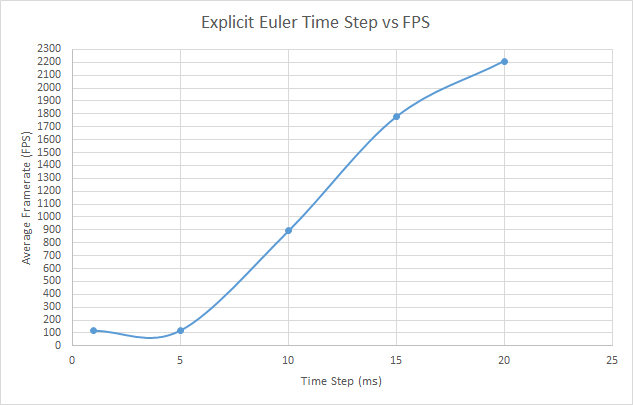
\includegraphics[scale=.9]{Figures/flag_ee_ts_fps}
    \end{center}
    \caption{Explicit Euler time step against average FPS for a 300 by 300 mesh (flag)}
    \label{fig:ee step fps flag}
  \end{figure}
  
    \begin{figure}
    \begin{center}
      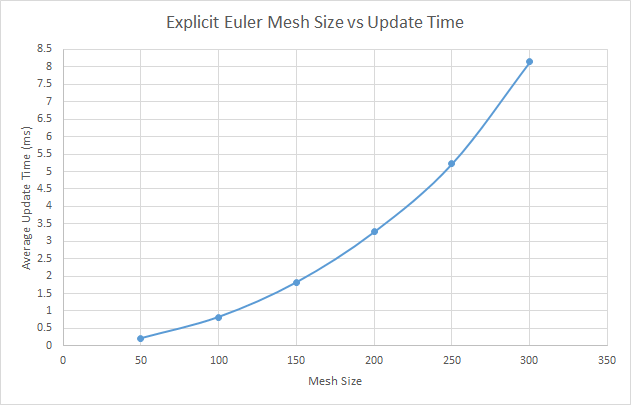
\includegraphics[scale=.9]{Figures/flag_ee_m_ut}
    \end{center}
    \caption{Explicit Euler mesh size against average update time (flag)}
    \label{fig:ee mesh update flag}
  \end{figure}
  
    \begin{figure}
    \begin{center}
      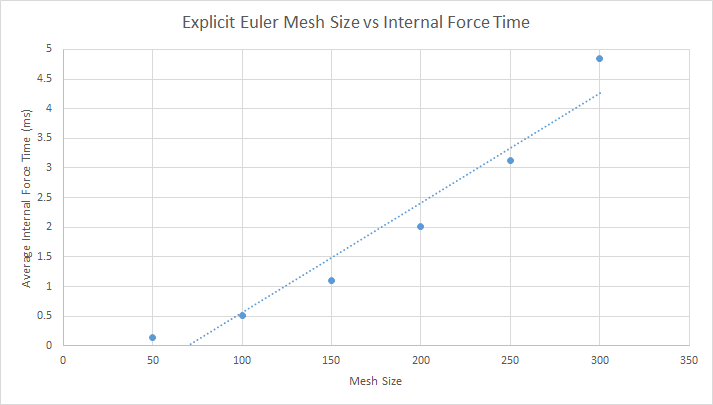
\includegraphics[scale=.9]{Figures/flag_ee_m_csf}
    \end{center}
    \caption{Explicit Euler mesh size against average internal force time (flag)}
    \label{fig:ee mesh csf flag}
  \end{figure}
  
    \begin{figure}
    \begin{center}
      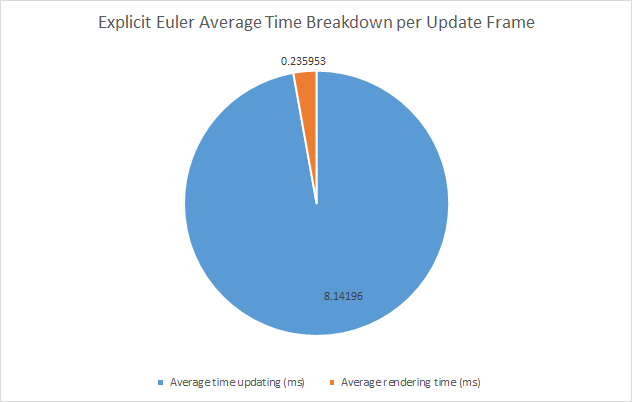
\includegraphics[scale=.9]{Figures/flag_ee_ft}
    \end{center}
    \caption{Explicit Euler frame time breakdown (flag)}
    \label{fig:ee ft flag}
  \end{figure}
  
    \begin{figure}
    \begin{center}
      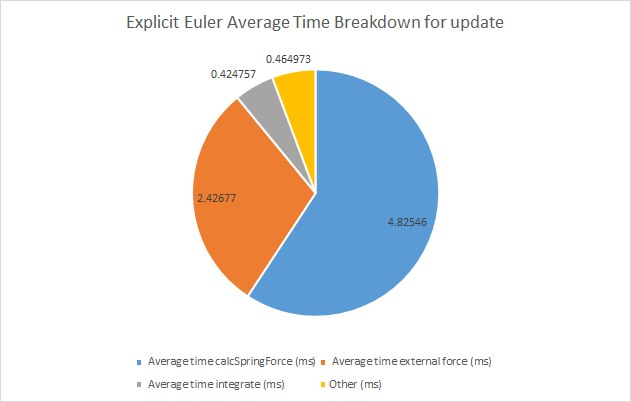
\includegraphics[scale=.9]{Figures/flag_ee_ut}
    \end{center}
    \caption{Explicit Euler update time breakdown (flag)}
    \label{fig:ee ut flag}
  \end{figure}

\begin{landscape}
\section{Verlet}

\subsection{Sheet Data}

  \begin{figure}[!htb]
    \begin{center}
      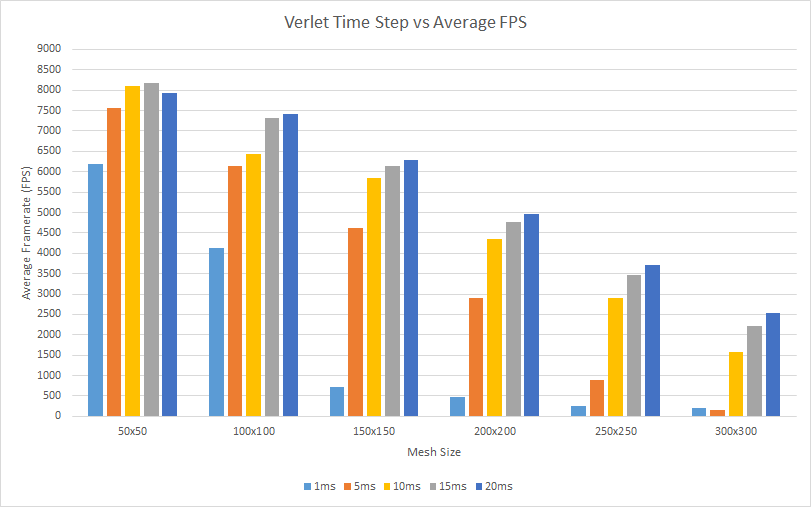
\includegraphics{Figures/sheet_v_fps}
    \end{center}
    \caption{Verlet time step against average FPS (sheet)}
    \label{fig:v fps sheet}
  \end{figure}
\end{landscape}
  
    \begin{figure}
    \begin{center}
      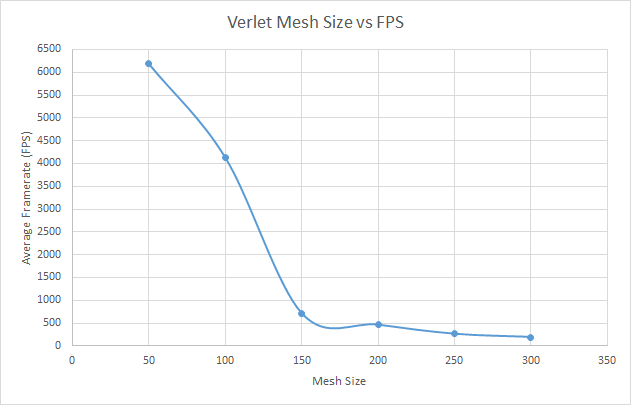
\includegraphics[scale=.9]{Figures/sheet_v_m_fps}
    \end{center}
    \caption{Verlet mesh size against average FPS (sheet)}
    \label{fig:v mesh fps sheet}
  \end{figure}
  
    \begin{figure}
    \begin{center}
      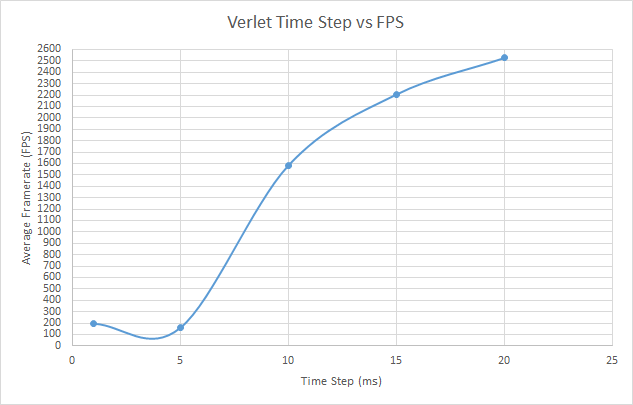
\includegraphics[scale=.9]{Figures/sheet_v_ts_fps}
    \end{center}
    \caption{Verlet time step against average FPS for a 300 by 300 mesh (sheet)}
    \label{fig:v step fps sheet}
  \end{figure}
  
    \begin{figure}
    \begin{center}
      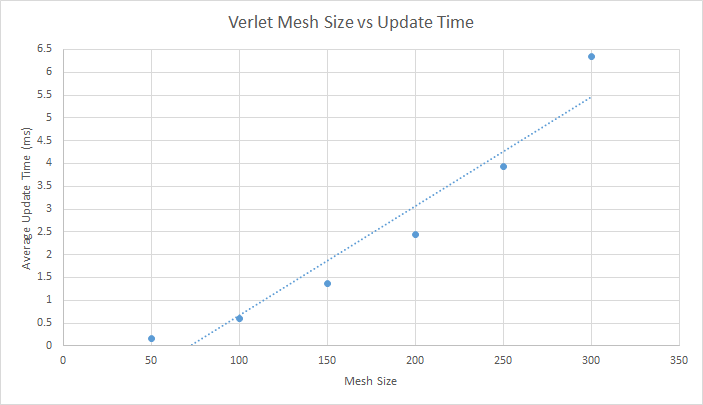
\includegraphics[scale=.9]{Figures/sheet_v_m_ut}
    \end{center}
    \caption{Verlet mesh size against average update time (sheet)}
    \label{fig:v mesh update sheet}
  \end{figure}
  
    \begin{figure}
    \begin{center}
      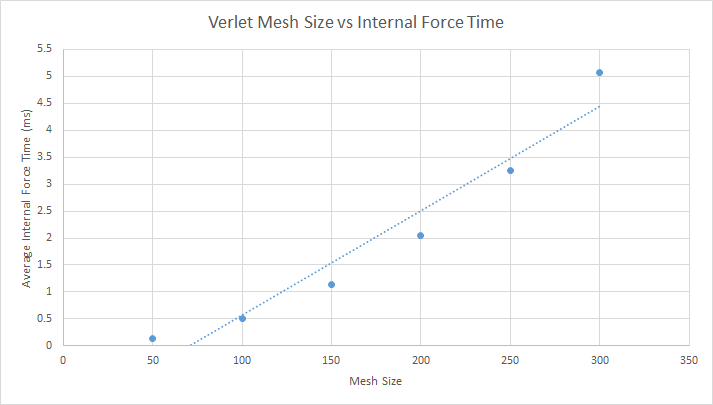
\includegraphics[scale=.9]{Figures/sheet_v_m_csf}
    \end{center}
    \caption{Verlet mesh size against average internal force time (sheet)}
    \label{fig:v mesh csf sheet}
  \end{figure}
  
    \begin{figure}
    \begin{center}
      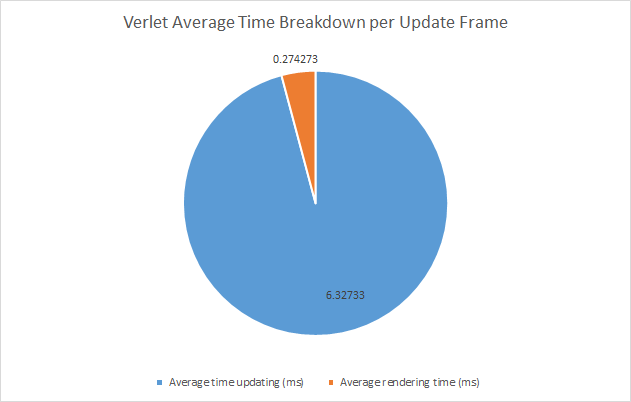
\includegraphics[scale=.9]{Figures/sheet_v_ft}
    \end{center}
    \caption{Verlet frame time breakdown (sheet)}
    \label{fig:v ft sheet}
  \end{figure}
  
    \begin{figure}
    \begin{center}
      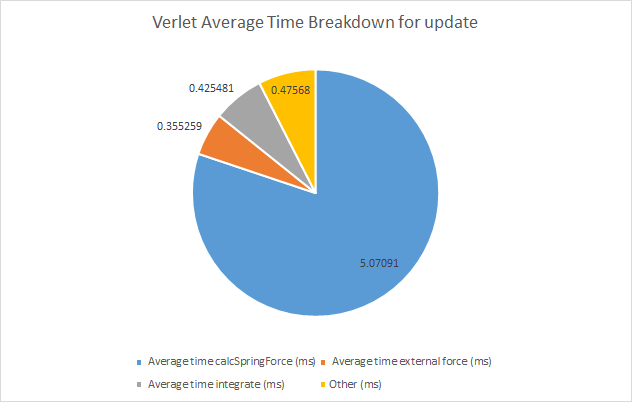
\includegraphics[scale=.9]{Figures/sheet_v_ut}
    \end{center}
    \caption{Verlet update time breakdown (sheet)}
    \label{fig:v ut sheet}
  \end{figure}

\begin{landscape}
\subsection{Flag Data}

    \begin{figure}[!htb]
    \begin{center}
      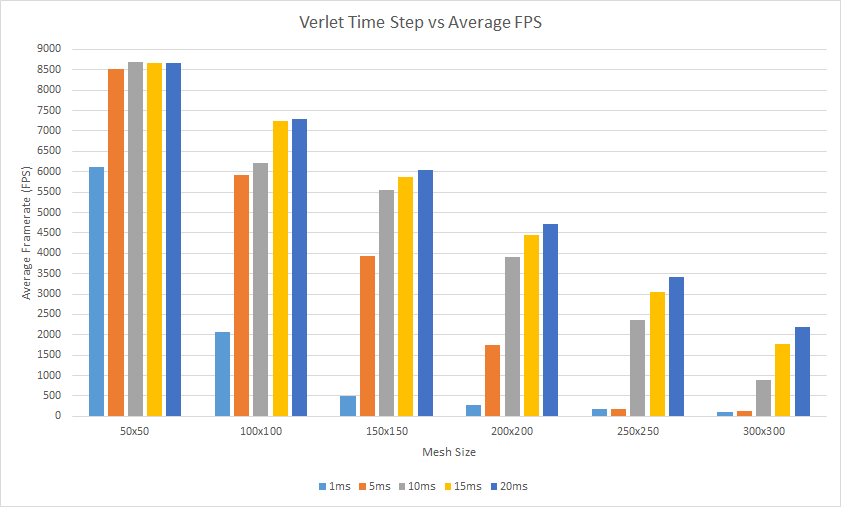
\includegraphics[scale=0.95]{Figures/flag_v_fps}
    \end{center}
    \caption{Verlet mesh size against average FPS (flag)}
    \label{fig:v fps flag}
  \end{figure}
\end{landscape}
  
    \begin{figure}
    \begin{center}
      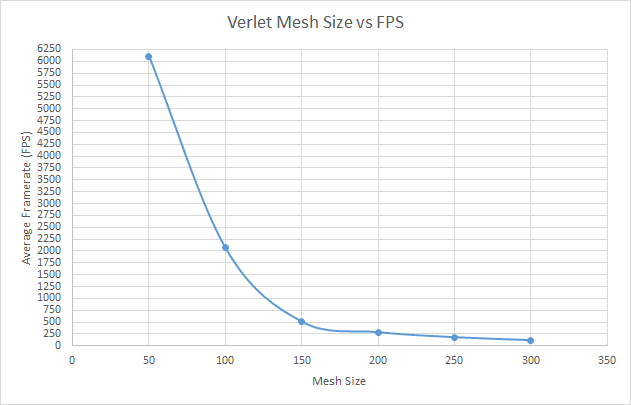
\includegraphics[scale=.9]{Figures/flag_v_m_fps}
    \end{center}
    \caption{Verlet mesh size against average FPS (flag)}
    \label{fig:v mesh fps flag}
  \end{figure}
  
    \begin{figure}
    \begin{center}
      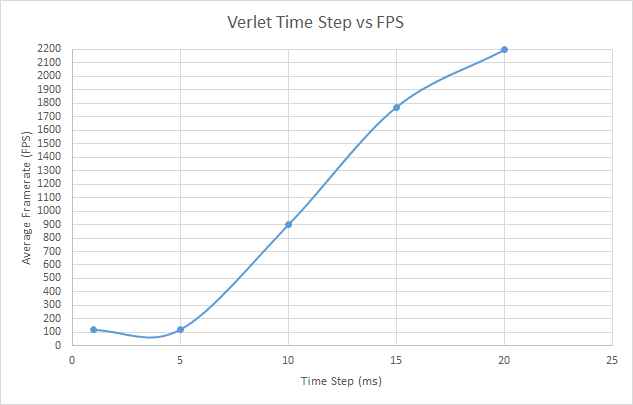
\includegraphics[scale=.9]{Figures/flag_v_ts_fps}
    \end{center}
    \caption{Verlet time step against average FPS for a 300 by 300 mesh (flag)}
    \label{fig:v step fps flag}
  \end{figure}
  
    \begin{figure}
    \begin{center}
      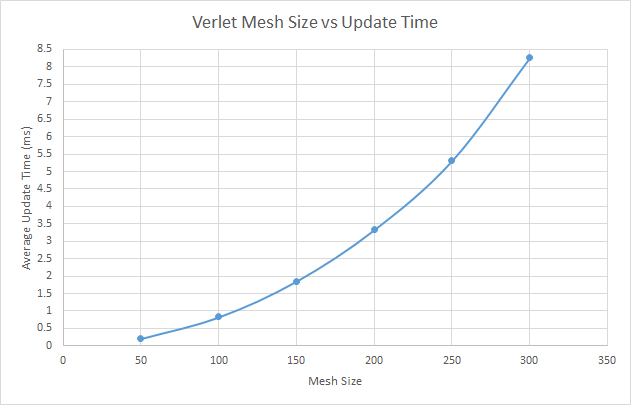
\includegraphics[scale=.9]{Figures/flag_v_m_ut}
    \end{center}
    \caption{Verlet mesh size against average update time (flag)}
    \label{fig:v mesh update flag}
  \end{figure}
  
    \begin{figure}
    \begin{center}
      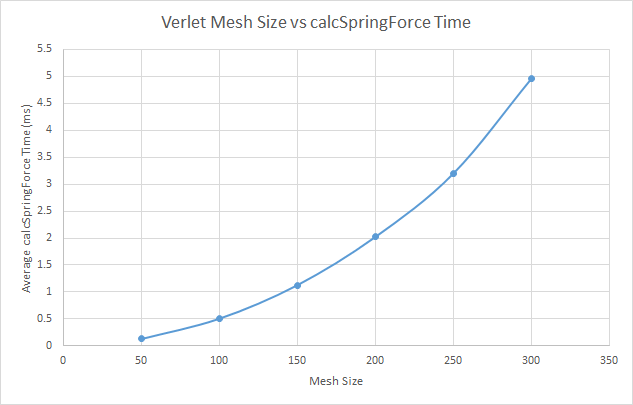
\includegraphics[scale=.9]{Figures/flag_v_m_csf}
    \end{center}
    \caption{Verlet mesh size against average internal force time (flag)}
    \label{fig:v mesh csf flag}
  \end{figure}
  
    \begin{figure}
    \begin{center}
      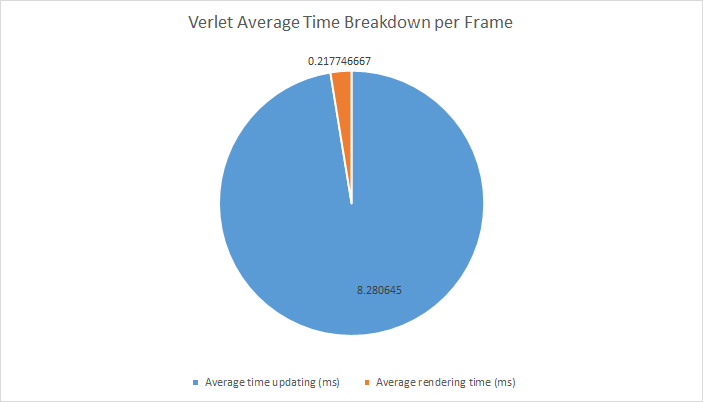
\includegraphics[scale=.9]{Figures/flag_v_ft}
    \end{center}
    \caption{Verlet frame time breakdown (flag)}
    \label{fig:v ft flag}
  \end{figure}
  
    \begin{figure}
    \begin{center}
      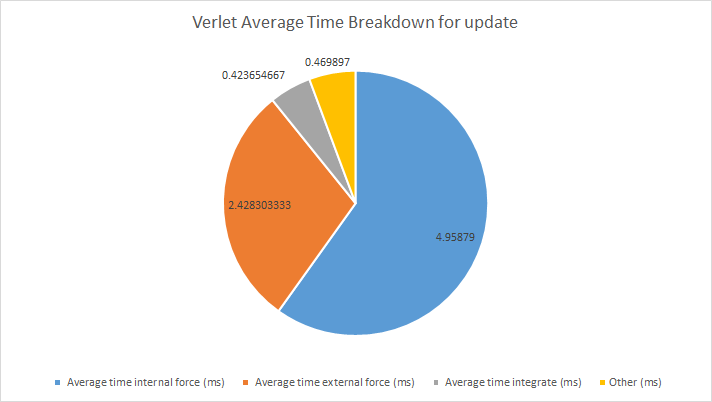
\includegraphics[scale=.9]{Figures/flag_v_ut}
    \end{center}
    \caption{Verlet update time breakdown (flag)}
    \label{fig:v ut flag}
  \end{figure}

\begin{landscape}
\section{Midpoint}

\subsection{Sheet Data}

  \begin{figure}[!htb]
    \begin{center}
      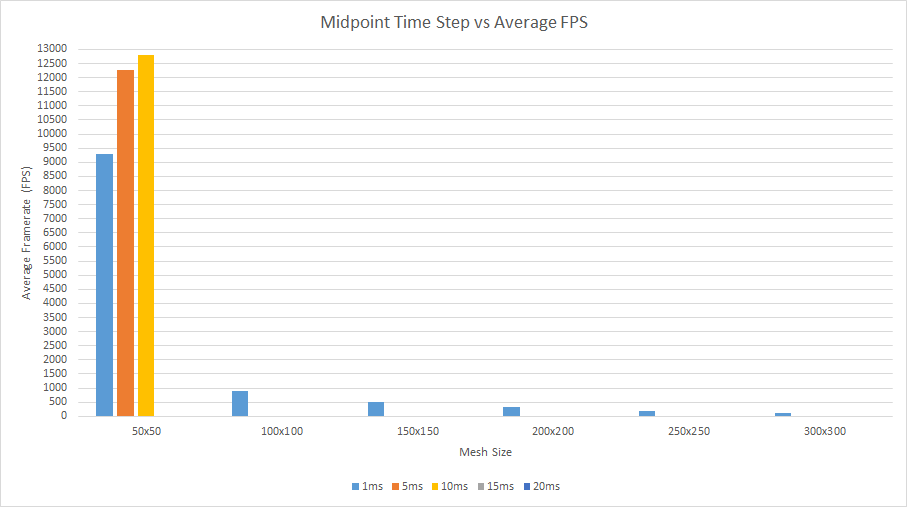
\includegraphics{Figures/sheet_m_fps}
    \end{center}
    \caption{Midpoint time step against average FPS (sheet)}
    \label{fig:m fps sheet}
  \end{figure}
\end{landscape}
  
    \begin{figure}
    \begin{center}
      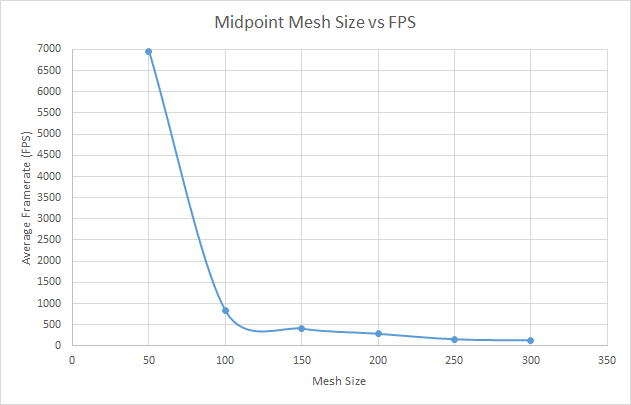
\includegraphics[scale=.9]{Figures/sheet_m_m_fps}
    \end{center}
    \caption{Midpoint mesh size against average FPS (sheet)}
    \label{fig:m mesh fps sheet}
  \end{figure}
  
    \begin{figure}
    \begin{center}
      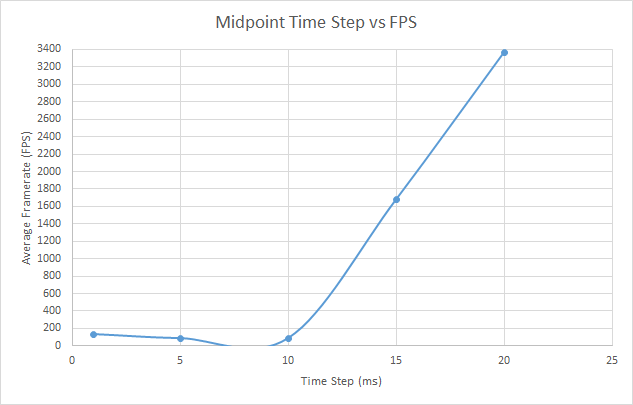
\includegraphics[scale=.9]{Figures/sheet_m_ts_fps}
    \end{center}
    \caption{Midpoint time step against average FPS for a 300 by 300 mesh (sheet)}
    \label{fig:m step fps sheet}
  \end{figure}
  
    \begin{figure}
    \begin{center}
      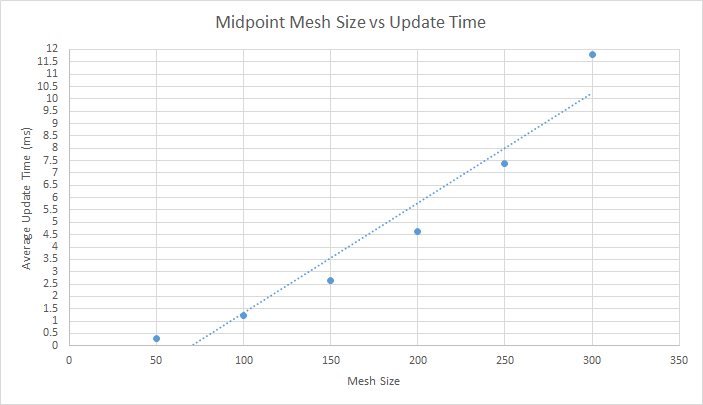
\includegraphics[scale=.9]{Figures/sheet_m_m_ut}
    \end{center}
    \caption{Midpoint mesh size against average update time (sheet)}
    \label{fig:m mesh update sheet}
  \end{figure}
  
    \begin{figure}
    \begin{center}
      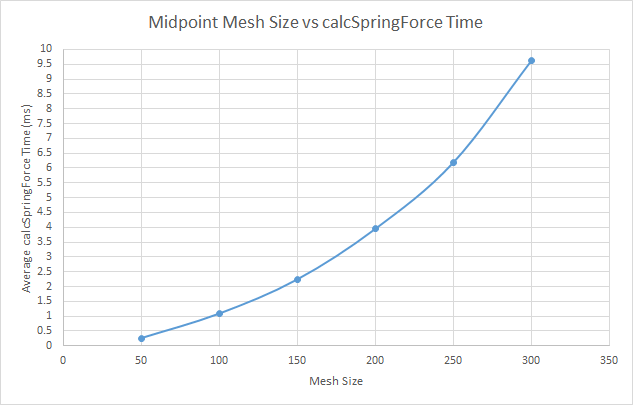
\includegraphics[scale=.9]{Figures/sheet_m_m_csf}
    \end{center}
    \caption{Midpoint mesh size against average internal force time (sheet)}
    \label{fig:m mesh csf sheet}
  \end{figure}
  
    \begin{figure}
    \begin{center}
      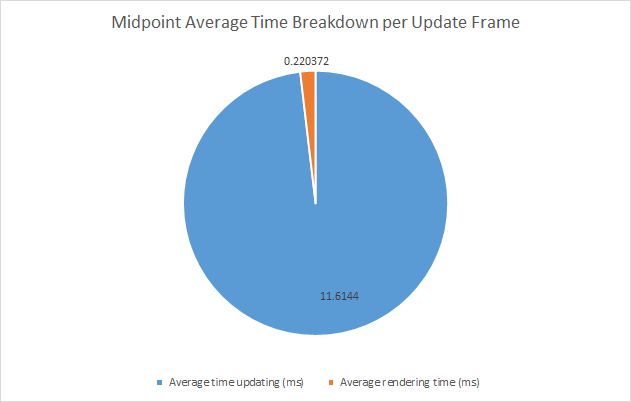
\includegraphics[scale=.9]{Figures/sheet_m_ft}
    \end{center}
    \caption{Midpoint frame time breakdown (sheet)}
    \label{fig:m ft sheet}
  \end{figure}
  
    \begin{figure}
    \begin{center}
      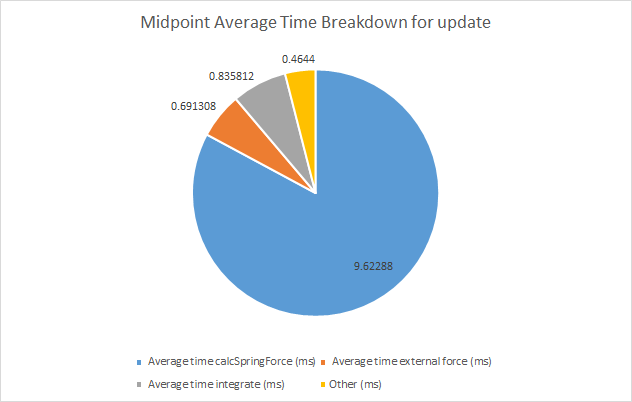
\includegraphics[scale=.9]{Figures/sheet_m_ut}
    \end{center}
    \caption{Midpoint update time breakdown (sheet)}
    \label{fig:m ut sheet}
  \end{figure}

\begin{landscape}
\subsection{Flag Data}

    \begin{figure}[!htb]
    \begin{center}
      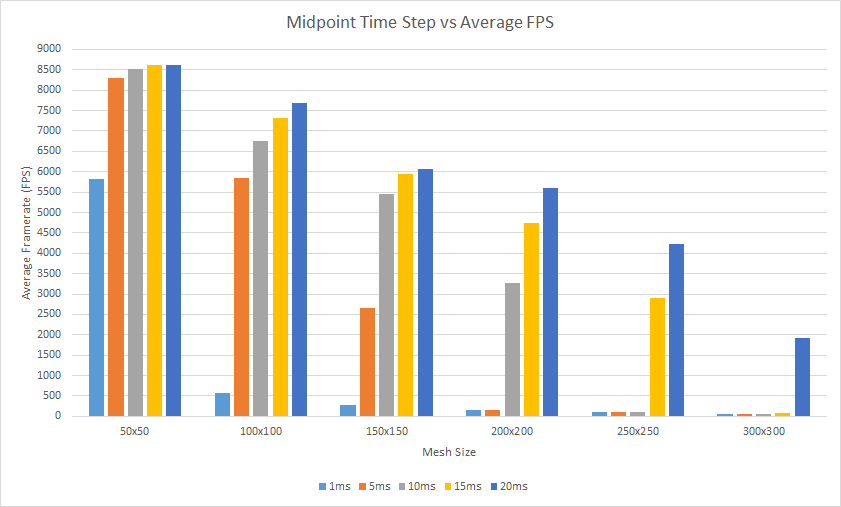
\includegraphics[scale=0.95]{Figures/flag_m_fps}
    \end{center}
    \caption{Midpoint mesh size against average FPS (flag)}
    \label{fig:m fps flag}
  \end{figure}
\end{landscape}
  
    \begin{figure}
    \begin{center}
      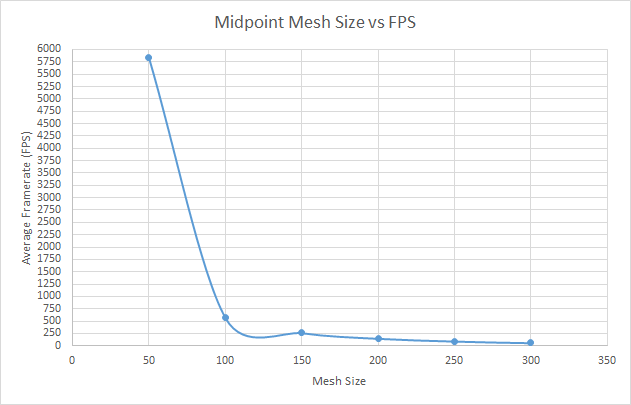
\includegraphics[scale=.9]{Figures/flag_m_m_fps}
    \end{center}
    \caption{Midpoint mesh size against average FPS (flag)}
    \label{fig:m mesh fps flag}
  \end{figure}
  
    \begin{figure}
    \begin{center}
      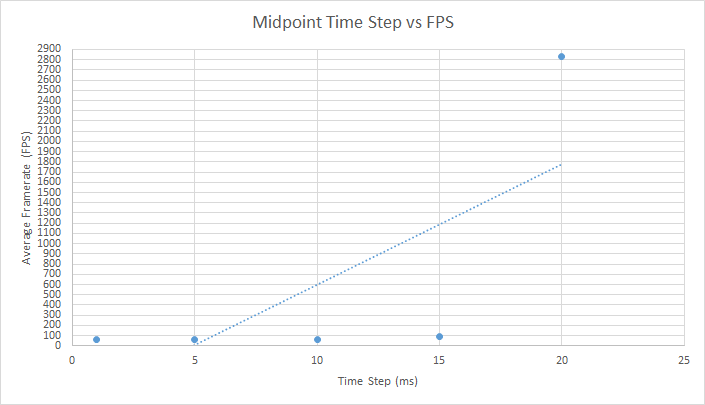
\includegraphics[scale=.9]{Figures/flag_m_ts_fps}
    \end{center}
    \caption{Midpoint time step against average FPS for a 300 by 300 mesh (flag)}
    \label{fig:m step fps flag}
  \end{figure}
  
    \begin{figure}
    \begin{center}
      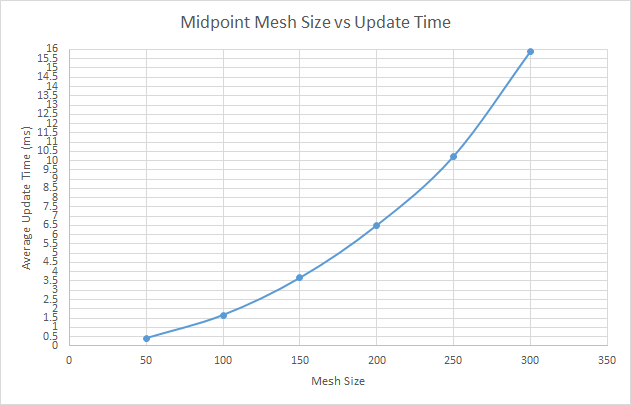
\includegraphics[scale=.9]{Figures/flag_m_m_ut}
    \end{center}
    \caption{Midpoint mesh size against average update time (flag)}
    \label{fig:m mesh update flag}
  \end{figure}
  
    \begin{figure}
    \begin{center}
      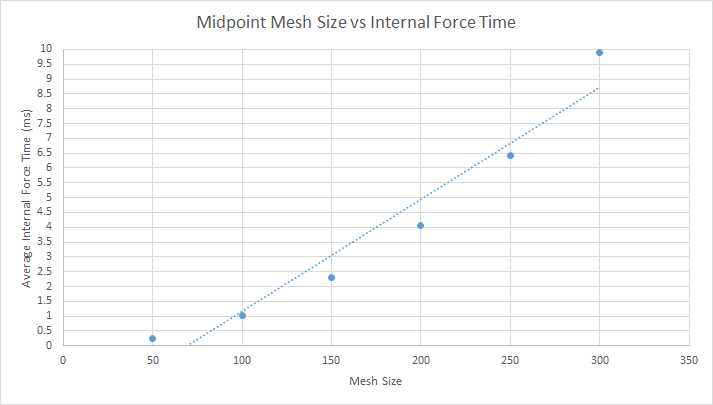
\includegraphics[scale=.9]{Figures/flag_m_m_csf}
    \end{center}
    \caption{Midpoint mesh size against average internal force time (flag)}
    \label{fig:m mesh csf flag}
  \end{figure}
  
    \begin{figure}
    \begin{center}
      \includegraphics[scale=.9]{Figures/flag_m_ft}
    \end{center}
    \caption{Midpoint frame time breakdown (flag)}
    \label{fig:m ft flag}
  \end{figure}
  
    \begin{figure}
    \begin{center}
      \includegraphics[scale=.9]{Figures/flag_m_ut}
    \end{center}
    \caption{Midpoint update time breakdown (flag)}
    \label{fig:m ut flag}
  \end{figure}

\begin{landscape}

\section{Fourth Order Runge-Kutta}

\subsection{Sheet Data}

  \begin{figure}[!htb]
    \begin{center}
      \includegraphics{Figures/sheet_rk4_fps}
    \end{center}
    \caption{Fourth Order Runge-Kutta time step against average FPS (sheet)}
    \label{fig:rk4 fps sheet}
  \end{figure}
\end{landscape}
  
    \begin{figure}
    \begin{center}
      \includegraphics[scale=.9]{Figures/sheet_rk4_m_fps}
    \end{center}
    \caption{Fourth Order Runge-Kutta mesh size against average FPS (sheet)}
    \label{fig:rk4 mesh fps sheet}
  \end{figure}
  
    \begin{figure}
    \begin{center}
      \includegraphics[scale=.9]{Figures/sheet_rk4_ts_fps}
    \end{center}
    \caption{Fourth Order Runge-Kutta time step against average FPS for a 300 by 300 mesh (sheet)}
    \label{fig:rk4 step fps sheet}
  \end{figure}
  
    \begin{figure}
    \begin{center}
      \includegraphics[scale=.9]{Figures/sheet_rk4_m_ut}
    \end{center}
    \caption{Fourth Order Runge-Kutta mesh size against average update time (sheet)}
    \label{fig:rk4 mesh update sheet}
  \end{figure}
  
    \begin{figure}
    \begin{center}
      \includegraphics[scale=.9]{Figures/sheet_rk4_m_csf}
    \end{center}
    \caption{Fourth Order Runge-Kutta mesh size against average internal force time (sheet)}
    \label{fig:rk4 mesh csf sheet}
  \end{figure}
  
    \begin{figure}
    \begin{center}
      \includegraphics[scale=.9]{Figures/sheet_rk4_ft}
    \end{center}
    \caption{Fourth Order Runge-Kutta frame time breakdown (sheet)}
    \label{fig:rk4 ft sheet}
  \end{figure}
  
    \begin{figure}
    \begin{center}
      \includegraphics[scale=.9]{Figures/sheet_rk4_ut}
    \end{center}
    \caption{Fourth Order Runge-Kutta update time breakdown (sheet)}
    \label{fig:rk4 ut sheet}
  \end{figure}

\begin{landscape}
\subsection{Flag Data}

    \begin{figure}[!htb]
    \begin{center}
      \includegraphics[scale=0.95]{Figures/flag_rk4_fps}
    \end{center}
    \caption{Fourth Order Runge-Kutta mesh size against average FPS (flag)}
    \label{fig:rk4 fps flag}
  \end{figure}
\end{landscape}
  
    \begin{figure}
    \begin{center}
      \includegraphics[scale=.9]{Figures/flag_rk4_m_fps}
    \end{center}
    \caption{Fourth Order Runge-Kutta mesh size against average FPS (flag)}
    \label{fig:rk4 mesh fps flag}
  \end{figure}
  
    \begin{figure}
    \begin{center}
      \includegraphics[scale=.9]{Figures/flag_rk4_ts_fps}
    \end{center}
    \caption{Fourth Order Runge-Kutta time step against average FPS for a 300 by 300 mesh (flag)}
    \label{fig:rk4 step fps flag}
  \end{figure}
  
    \begin{figure}
    \begin{center}
      \includegraphics[scale=.9]{Figures/flag_rk4_m_ut}
    \end{center}
    \caption{Fourth Order Runge-Kutta mesh size against average update time (flag)}
    \label{fig:rk4 mesh update flag}
  \end{figure}
  
    \begin{figure}
    \begin{center}
      \includegraphics[scale=.9]{Figures/flag_rk4_m_csf}
    \end{center}
    \caption{Fourth Order Runge-Kutta mesh size against average internal force time (flag)}
    \label{fig:rk4 mesh csf flag}
  \end{figure}
  
    \begin{figure}
    \begin{center}
      \includegraphics[scale=.9]{Figures/flag_rk4_ft}
    \end{center}
    \caption{Fourth Order Runge-Kutta frame time breakdown (flag)}
    \label{fig:rk4 ft flag}
  \end{figure}
  
    \begin{figure}
    \begin{center}
      \includegraphics[scale=.9]{Figures/flag_rk4_ut}
    \end{center}
    \caption{Fourth Order Runge-Kutta update time breakdown (flag)}
    \label{fig:rk4 ut flag}
  \end{figure}

\begin{landscape}

\section{All Integrators}

\subsection{Sheet Data}

    \begin{figure}[!htb]
    \begin{center}
      \includegraphics{Figures/sheet_1ms_int_fps}
    \end{center}
    \caption{Mesh size against average FPS for all integrators with 1ms time step (sheet)}
    \label{fig:1ms fps sheet}
  \end{figure}
  
    \begin{figure}[!htb]
    \begin{center}
      \includegraphics{Figures/sheet_5ms_int_fps}
    \end{center}
    \caption{Mesh size against average FPS for all integrators with 5ms time step (sheet)}
    \label{fig:5ms fps sheet}
  \end{figure}
  
    \begin{figure}[!htb]
    \begin{center}
      \includegraphics{Figures/sheet_10ms_int_fps}
    \end{center}
    \caption{Mesh size against average FPS for all integrators with 10ms time step (sheet)}
    \label{fig:10ms fps sheet}
  \end{figure}

    \begin{figure}[!htb]
    \begin{center}
      \includegraphics{Figures/sheet_15ms_int_fps}
    \end{center}
    \caption{Mesh size against average FPS for all integrators with 15ms time step (sheet)}
    \label{fig:15ms fps sheet}
  \end{figure}
  
    \begin{figure}[!htb]
    \begin{center}
      \includegraphics{Figures/sheet_20ms_int_fps}
    \end{center}
    \caption{Mesh size against average FPS for all integrators with 20ms time step (sheet)}
    \label{fig:20ms fps sheet}
  \end{figure}
  
    \begin{figure}[!htb]
    \begin{center}
      \includegraphics{Figures/sheet_int_ut}
    \end{center}
    \caption{Average update time for each integrator (sheet)}
    \label{fig:ut sheet}
  \end{figure}

\end{landscape}

\begin{landscape}
\subsection{Flag Data}

    \begin{figure}[!htb]
    \begin{center}
      \includegraphics[scale=0.95]{Figures/flag_1ms_int_fps}
    \end{center}
    \caption{Mesh size against average FPS for all integrators with 1ms time step (flag)}
    \label{fig:1ms fps flag}
  \end{figure}
  
    \begin{figure}[!htb]
    \begin{center}
      \includegraphics{Figures/flag_5ms_int_fps}
    \end{center}
    \caption{Mesh size against average FPS for all integrators with 5ms time step (flag)}
    \label{fig:5ms fps flag}
  \end{figure}
  
    \begin{figure}[!htb]
    \begin{center}
      \includegraphics{Figures/flag_10ms_int_fps}
    \end{center}
    \caption{Mesh size against average FPS for all integrators with 10ms time step (flag)}
    \label{fig:10ms fps flag}
  \end{figure}

    \begin{figure}[!htb]
    \begin{center}
      \includegraphics{Figures/flag_15ms_int_fps}
    \end{center}
    \caption{Mesh size against average FPS for all integrators with 15ms time step (flag)}
    \label{fig:15ms fps flag}
  \end{figure}
  
    \begin{figure}[!htb]
    \begin{center}
      \includegraphics{Figures/flag_20ms_int_fps}
    \end{center}
    \caption{Mesh size against average FPS for all integrators with 20ms time step (flag)}
    \label{fig:20ms fps flag}
  \end{figure}
  
    \begin{figure}[!htb]
    \begin{center}
      \includegraphics{Figures/flag_int_ut}
    \end{center}
    \caption{Average update time for each integrator (flag)}
    \label{fig:ut flag}
  \end{figure}
  
\end{landscape}